\documentclass[10pt]{article}
\usepackage[utf8]{inputenc}
\usepackage[T1]{fontenc}
\usepackage{amsmath}
\usepackage{amsfonts}
\usepackage{amssymb}
\usepackage[version=4]{mhchem}
\usepackage{stmaryrd}
\usepackage{graphicx}
\usepackage[export]{adjustbox}
\graphicspath{ {./images/} }

\begin{document}
\begin{enumerate}
  \item The graph below shows the velocity $v$ in metres per second of a particle at time $t$ seconds.\\
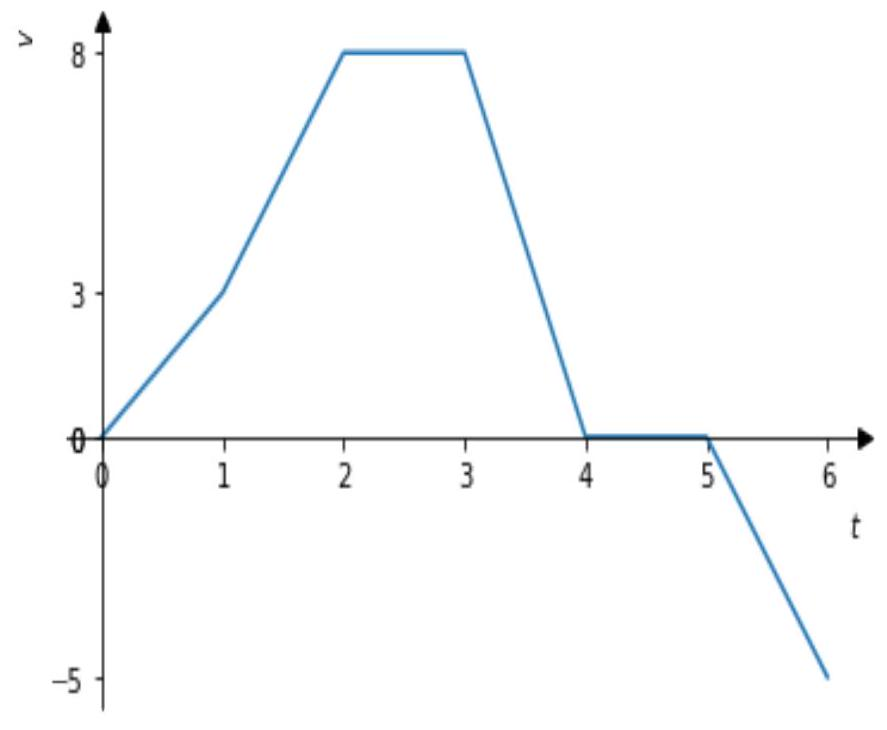
\includegraphics[max width=\textwidth, center]{2024_12_26_56998f94318d3dea0eedg-1}\\
(a) Describe the motion of this particle. When is it moving forwards? When is it accelerating? When is it decelerating?\\
(b) Express the velocity $v(t)$ as a function of $t$.\\
(c) Sketch a graph of the acceleration of this particle.\\
(d) Express the acceleration $a(t)$ of the particle as a function of $t$\\
(e) Sketch a graph for the position of this particle.\\
(f) Bonus: Express the position $s(t)$ as a function of $t$, where the position of the function at time $t=0$ is 0 . i.e. $s(0)=0$.
  \item Suppose we have a circle inscribed in a square.\\
(a) If the perimeter of the square is increasing at a rate of $10 \mathrm{~m} / \mathrm{s}$, at what rate is the circumference of the circle increasing?\\
(b) If the area of the circle is increasing at a rate of $10 \mathrm{~m}^{2} / \mathrm{s}$, at what rate is the diagonal of the square increasing when the area of the circle is $\pi$ ?
  \item If $\$ 1500$ is borrowed at $8 \%$ interest, find the amounts due at the end of 5 years if the interest is compounded:\\
(a) annually;\\
(b) monthly;\\
(c) daily;\\
(d) continuously.
\end{enumerate}

Hint: Have a look at Section 3.8, Example 3 in the textbook.\\
4. Recall that the rate of cooling of an object is proportional to the difference in temperature between the object and its surrounding.\\
A freshly brewed cup of coffee has temperature $95^{\circ} \mathrm{C}$ in a $20^{\circ} \mathrm{C}$ room. When its temperature is $70^{\circ} \mathrm{C}$, it is cooling at a rate of $1^{\circ} \mathrm{C}$ per minute. When does this occur?\\
5. Two cars start moving from the same point. One travels south at $60 \mathrm{~km} / \mathrm{h}$ and the other travel west at $25 \mathrm{~km} / \mathrm{h}$. At what rate is the distance between the cars increasing two hours later?\\
6. A particle is moving along the curve $y=\sqrt{x}$. As the particle passes through the point $(4,2)$, its $x$-coordinate increases at a rate of 3 units $/ \mathrm{s}$. How fast is its $y$-coordinate changing at this instant? Hint: think of the coordinates as functions of time, $y=y(t)$ and $x=x(t)$; what can you say about the coordinates of the particle at time $t$ ?.


\end{document}